\chapter{Balanced decorations of simple white spheres}
\label{ch:balanced-terminal-fans}

The tree constructions are not the only diagrams whose full invariant
can be controlled. This chapter starts with an arbitrary connected
marked augmented diagram whose white faces form a simple triangulated
sphere. The diagram may have cyclic couplings in its finite source.
We add finitely many terminal tangles near each crossing circle and
prove the volume limit for the resulting knots after independently
sufficiently long fixed fillings.

The construction has a geometric purpose. It leaves every old circle
in the complete packing fixed and adds disks in its triangular gaps.
By choosing the numbers of insertions on the two sides separately,
one obtains a strict inequality at the same complete packing for every
crossing circle. This bounds the one-sided terms of the full spectral
numerator below the geometric contribution. The knot being evaluated
is the decorated knot, with all its original and added circles filled;
it need not be isotopic to the initial core knot.

\section{The diagrams and the result}

Cut an augmented diagram along its projection regions and its
twice-punctured crossing disks. The pieces of the projection regions
are called white faces. Each crossing disk contributes two shaded
triangles, paired with one another. The dual description has one
vertex for each white region and one triangle for each shaded face.
The side shared by a paired pair of triangles is its matching edge.
These are incidence data of the given diagram, including its cyclic
orders, rather than a graph selected afterward to model its source.

Require this white cellulation to be a simple triangulated sphere with
at least four vertices. Thus every triangular cell has three distinct
vertices, and there are no loops or repeated edges. A strand edge is a side not used in the matching. Keep one original
strand edge for the reduced mark; its endpoints are the two protected
faces in the finite coefficient formula. The diagram can be a general Morse diagram:
ordinary cups and caps are allowed between its crossing boxes.

\begin{theorem}[Balanced terminal decoration]
\label{bf:volume-theorem}
Fix such a diagram, its crossing-disk frames, and a parity pattern
whose main strands form one knot. There is a finite decoration by
terminal crossing-circle tangles, with an even number added on each
side of every original crossing box, with the following property.
For the resulting fixed augmented diagram $\widehat D$ there is a
threshold $P(\widehat D)$ such that every fixed independently signed
integer filling vector with $|p_e|\ge P(\widehat D)$ gives
\begin{equation}\label{bf:volume}
 \lim_{N\to\infty}\frac{2\pi}{N}\log|K_N(K_{\mathbf p})|
             =\Vol(S^3\setminus K_{\mathbf p}).
\end{equation}
The physical crossing powers are $n_e=\epsilon_e-2p_e$ in their
recorded disk frames. Each added terminal has odd parity. The endpoint
pairing remains a knot, the filled complement is hyperbolic, and the
limit includes both parities and composite levels.
\end{theorem}

The decorations and all the powers are fixed before $N$ tends to
infinity. The threshold depends on the final diagram; it imposes no
ratio bound on the different powers. In particular the original boxes
are also filled sufficiently long. This is not a statement about
arbitrary short fillings or about the invariant of the undecorated
core. It concerns the complete main color, without a new moving
main-meridian or operator conclusion.

There is also a wholly combinatorial way to supply starting diagrams.
Take any finite oriented simple triangulated sphere with at least four
vertices and a chosen perfect matching of its cubic dual. Each matched
pair is a disk with four distinct boundary vertices. Place the standard
crossing-circle box there and join its four terminals along the
remaining embedded dual edges. This constructs a link in $S^3$ with
the stated cut. A spanning tree in the incidence graph of its untwisted
main circles specifies odd boxes that merge those circles into one knot.
The signs at these odd boxes may be chosen independently. Theorem
\ref{bf:volume-theorem} then applies after the terminal decoration.

\section{A circle packing from the finite combinatorics}

No additional positive polyhedron is an unverified input. Remove one
triangle of the white sphere and prescribe three positive boundary
circle radii. The remaining disk has a strictly positive angle
assignment with demand $2\pi$ at each interior vertex and total
boundary demand $\pi$. The proof is a finite Hall count: every proper
interior subset touches strictly more triangle supply than its demand,
and the same holds for a subset containing the pooled boundary.
Separating triangles are allowed.

The strictly concave triangle entropy has an interior maximum on this
angle polytope. Its multipliers give radii and Euclidean triangles with
side lengths $r_f+r_g$. Their interior angle sums are $2\pi$, so their
development is locally Euclidean. The boundary goes once around the
prescribed convex triangle. The winding-number argument makes the
development an embedding. The disk sectors stop strictly before the
opposite center edge in every triangle, which excludes unintended
circle contacts. The contact circles of the triangular gaps supply
all shaded supporting planes. Together with the white planes they
bound the labeled convex ideal right-angled polyhedron.

The original projection and disk-face maps glue two copies into the
actual augmented exterior. Canonical cusp decorations make every
right-angle edge cycle and cusp complete. Sending the marked strand-edge
contact to infinity gives two parallel marked white lines and positive
finite curvatures at all other white faces. Appendix
\ref{app:balanced-terminal-fans} proves this construction, including
the support inequalities and the primitive marking.

\section{How two fans produce the needed inequality}

At one crossing circle let the paired triangles have white curvatures
$(x,b,y)$ and $(x,c,y)$, with matching edge $xy$. Put
\begin{equation}\label{bf:fan-parameters}
 A=x+y>0,\qquad P=xy,\qquad \rho=P/A^2\in[0,1/4].
\end{equation}
Inserting one terminal tangle in the first triangular gap introduces
the circle of curvature
\[
 b_1=A+b+2\sqrt{Ab+P}.
\]
The old matching edge $xy$ remains; its first middle face is now $b_1$.
The new matching edge is $bb_1$. Every old circle stays fixed.

\begin{figure}[htbp]
 \centering
 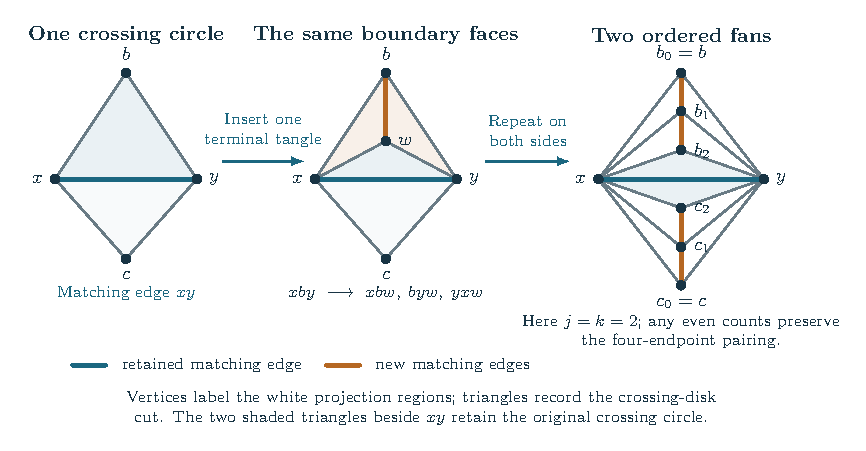
\includegraphics[width=\linewidth]{../book/figures/balanced-terminal-fans.pdf}
 \caption{A terminal insertion in the white-face triangulation and its
 repetition on both sides of one crossing circle. The retained matching
 edge is $xy$; the added matching edge is $bw$. The cyclic order of
 the new four-sided region is $(b,y,w,x)$, so the new source factor
 is $H_g(b,y,x,w)$. The drawing records the inherited cut and matching.
 Here $j=k=2$; any even counts preserve the four-endpoint pairing.}
 \label{fig:balanced-terminal-fans}
\end{figure}

The convexity of this insertion can be checked in a single explicit
model. Normalize the old white circles to two parallel lines at heights
zero and two and a unit disk centered at $i$. The right interstice
receives the unit disk centered at $2+i$. Its three new shaded disks
are $|z-1|<1$, $|z-(1+2i)|<1$, and $\Re z>2$, all contained in the old
shaded halfplane $\Re z>0$. The other old supporting inequalities
therefore remain strict at new nonincident contacts. Repeating the
construction gives nested gaps without intersections, including when
the global marked faces are lines.

The recurrence is exactly solvable:
\begin{equation}\label{bf:fan-recurrence}
 \sqrt{Ab_j+P}=\sqrt{Ab+P}+jA.
\end{equation}
Choose even nonnegative counts $j,k$ so that
\[
 U=\sqrt{b/A+\rho}+j\ge4,\qquad
 V=\sqrt{c/A+\rho}+k\ge4,\qquad |U-V|\le1.
\]
This is possible by rounding the difference to an even integer and
then adding the same sufficiently large even integer to both counts.

Let $F(x,b,y)$ be the source-normalized complete triangle action.
Its entropy formula fixes the constant in the useful identity
\begin{equation}\label{bf:remainder}
\begin{aligned}
 F(x,b,y)&=\tfrac12\log b+R(b),\\
 R(b)&=\frac1\pi\int_b^\infty
        \arctan\frac{\sqrt{At+P}}t\,\frac{dt}{t}.
\end{aligned}
\end{equation}
For $b_j=A(U^2-\rho)$ and $c_k=A(V^2-\rho)$, elementary estimates
of this positive remainder give
\begin{equation}\label{bf:strict-balance}
 F(x,b_j,y)+F(x,c_k,y)-\max(\log b_j,\log c_k)
     >\frac{3347}{27720\min(U,V)}>0.
\end{equation}
Every new crossing circle satisfies the simpler algebraic balance
test already at its creation: its outer sum is $b+b_1\ge x+y$ and
its two middle curvatures are $x,y$. Later insertions do not alter it.
Thus finitely many two-sided fans settle every original and added
crossing circle on one shared complete packing.

\section{The full finite source and the filled metric}

The diagram after insertion has additional intermediate cups and caps.
They must be evaluated in their inherited frames. For a first-side
insertion the two exact homogeneous factors are
\begin{equation}\label{bf:local-source}
             H_f(x,w,c,y)H_g(b,y,x,w).
\end{equation}
The face-winding identity preserves every old coefficient target and
gives the new ordinary target $N-1$. At even levels the new face has
the same parity clock as $b$. The extra factor $N^{-1}$ from its
coupon is cancelled by its new primitive face grid; the original
unrestricted mark is restricted only after whole-source conservation.
Consequently the full spectral numerator, including Casimir normals,
is the original marked coefficient on the refined diagram.

The part whose local cofactor paths cross the middle index has a
nonzero local geometric packet and a global spectral gap. These arguments use the simple
sphere, local cofactor estimates and shared Cauchy torus, with no
flat-plat sweep. Inequality \eqref{bf:strict-balance} bounds every
sector containing a one-sided term by a strictly smaller exponential
rate at those same radii. The original whole-domain Fourier/Hermite
filling formula retains its sine endpoints, parity signs and
second-derivative endpoint currents. Its first charge survives and
the remaining charges are smaller for independently long fixed powers.
This proves a nonzero asymptotic for the full invariant.

The geometric conclusion has a separate metric step. The common
deformed circle pattern and its full ordered collar maps give the
actual representation, with primitive logarithms
\[
 U_e=-\log R_{0,e}-\epsilon_e\log(-J_e),\qquad
 V_e=2\log(-J_e),\qquad U_e+p_eV_e=-2\pi i.
\]
For sufficiently long fixed powers it lies in a fixed neighborhood of
the complete framed representation. A positive equivariant developing
map on the compact core and a complete logarithmic cusp link identify
these logarithms with the actual periods. The primitive $2\pi$ angular
period completes the end to a smooth solid torus on the specified
slope. The main cusp remains complete. The regulator's boundary term
then cancels the filling phase and identifies the nonzero exponential
rate with the volume of this actual filled knot complement. The full
construction and estimates are given in Appendix
\ref{app:balanced-terminal-fans}.

The new tangles retain the correlations around cycles. On the graph
obtained by collapsing the source's physical cycles, one insertion
adds a loop. The proof controls those channels through the full shared
coefficient and its strict balance; it does not replace the invariant
by a scalar tree contraction.
